\documentclass[10pt,t]{beamer}
%\documentclass[c,mathserif,compress,xcolor=svgnames]{beamer} 
\usepackage[utf8]{inputenc}
\usepackage[T1]{fontenc}
\fontfamily{ppl}\selectfont

\usepackage{fontspec} 
\defaultfontfeatures{Mapping=tex-text} 
\setsansfont[Ligatures={Common}]{Futura}
\setmonofont[Scale=0.8]{Monaco} 


%\setbeamersize{text margin left=10pt,text margin right=10pt}
\usetheme{lehigh}

\usefonttheme{professionalfonts}
\usefonttheme{serif}

\pgfdeclarelayer{background}
\pgfdeclarelayer{foreground}
\pgfsetlayers{background,main,foreground}

% add packages to use
%\usepackage[latin1]{inputenc}
%\usepackage[english]{babel}
%\usepackage[normalem]{ulem}
\usepackage{times}
\usepackage[T1]{fontenc}
\usepackage{pgf,pgfarrows,pgfnodes,pgfautomata,pgfheaps,pgfshade}
\usepackage{amsmath,amssymb,amsfonts,subfigure,pifont}
\usepackage{graphicx}
\usepackage{multirow,multicol}
\usepackage{tabularx}
\usepackage{booktabs}
\usepackage{colortbl}
\usepackage{fancyvrb,listings}
\usepackage{algorithm,algpseudocode}
%\usepackage{keystroke}
\usepackage{etex}
\usepackage{hyperref}
\usepackage{tikz}
\usetikzlibrary{trees,matrix,shapes,arrows}
\usetikzlibrary{calc}



% The following color are for listing environment 
\definecolor{dkgreen}{rgb}{0,0.6,0}
\definecolor{DarkGreen}{rgb}{0.0,0.3,0.0}
\definecolor{gray}{rgb}{0.5,0.5,0.5}
\definecolor{mauve}{rgb}{0.58,0,0.82}
\definecolor{Blue}{rgb}{0.0,0.0,0.8} 
\definecolor{dodgerblue}{rgb}{0.1,0.1,1.0}
\definecolor{indigo}{rgb}{0.41,0.1,0.0}
\definecolor{seagreen}{rgb}{0.1,1.0,0.1}


\lstset{%
language=bash,                % the language of the code
basicstyle=\tiny\ttfamily,           % the size of the fonts that are used for the code
showspaces=false,               % show spaces adding particular underscores
showstringspaces=false,         % underline spaces within strings
showtabs=false,                 % show tabs within strings adding particular underscores
%frame=single,                   % adds a frame around the code
%rulecolor=\color{black},        % if not set, the frame-color may be changed on line-breaks within not-black text (e.g. comments (green here))
tabsize=2,                      % sets default tabsize to 2 spaces
%captionpos=b,                   % sets the caption-position to bottom
breaklines=true,                % sets automatic line breaking
breakatwhitespace=false,        % sets if automatic breaks should only happen at whitespace
%title=\lstname,                   % show the filename of files included with \lstinputlisting;
% also try caption instead of title
keywordstyle=\color{blue},          % keyword style
commentstyle=\color{dkgreen},       % comment style
stringstyle=\color{mauve},         % string literal style
escapeinside={!}{!},            % if you want to add LaTeX within your code
morekeywords={*,\dots,elif},              % if you want to add more keywords to the set
deletekeywords={\dots},              % if you want to delete keywords from the given language
%morecomment=[l]{//}
}
\lstset{%
language=csh,                % the language of the code
basicstyle=\tiny\ttfamily,           % the size of the fonts that are used for the code
showspaces=false,               % show spaces adding particular underscores
showstringspaces=false,         % underline spaces within strings
showtabs=false,                 % show tabs within strings adding particular underscores
%frame=single,                   % adds a frame around the code
%rulecolor=\color{black},        % if not set, the frame-color may be changed on line-breaks within not-black text (e.g. comments (green here))
tabsize=2,                      % sets default tabsize to 2 spaces
captionpos=b,                   % sets the caption-position to bottom
breaklines=true,                % sets automatic line breaking
breakatwhitespace=false,        % sets if automatic breaks should only happen at whitespace
%title=\lstname,                   % show the filename of files included with \lstinputlisting;
% also try caption instead of title
keywordstyle=\color{blue},          % keyword style
commentstyle=\color{dkgreen},       % comment style
stringstyle=\color{mauve},         % string literal style
escapeinside={\%*}{*)},            % if you want to add LaTeX within your code
morekeywords={*,\dots,elif},              % if you want to add more keywords to the set
deletekeywords={\dots},              % if you want to delete keywords from the given language
%morecomment=[l]{//}
}

\lstdefinestyle{LINUX}
{
    backgroundcolor=\color{white},
    basicstyle=\tiny\ttfamily,
    keywordstyle=\color{blue},
    morekeywords={apacheco,Tutorials,BASH,scripts,day1,examples},
    literate={>}{{\textcolor{blue}{>}}}1
         {/}{{\textcolor{blue}{/}}}1
         {./}{{\textcolor{black}{./ }}}1
         {~}{{\textcolor{blue}{\textasciitilde}}}1,
}

\lstdefinestyle{customc}{
  belowcaptionskip=1\baselineskip,
  breaklines=true,
  xleftmargin=\parindent,
  language=C,
  showstringspaces=false,
  basicstyle=\tiny\ttfamily,
  keywordstyle=\bfseries\color{green!40!black},
  commentstyle=\upshape\color{red!90!white},
  identifierstyle=\color{blue},
  stringstyle=\color{orange},
}
\lstdefinelanguage{OmpFortran}[]{Fortran}{
   rulesepcolor=\color{black},
   %
   extendedchars=true,
   %
   morecomment=[l] [\bfseries\color{red!90!white}]{!\$omp},
   morecomment=[l] [\bfseries\color{red!90!white}]{c\$omp},
   morecomment=[l] [\bfseries\color{red!90!white}]{*\$omp},
   morecomment=[l] [\bfseries\color{red!90!white}]{!\$acc},
   morecomment=[l] [\bfseries\color{red!90!white}]{c\$acc},
   morecomment=[l] [\bfseries\color{red!90!white}]{*\$acc},
}[comments]

\lstdefinelanguage{OmpC}[]{OmpFortran}{
   rulesepcolor=\color{black},
   %
   extendedchars=true,
   %
   morecomment=[l] [\bfseries\color{red!90!white}]{\#pragma\ omp},
   morecomment=[l] [\bfseries\color{red!90!white}]{\#pragma\ acc},
}[comments]

\lstset{escapechar=@,style=customc}
\lstset{literate=%
   *{0}{{{\color{blue}0}}}1
    {1}{{{\color{blue}1}}}1
    {2}{{{\color{blue}2}}}1
    {3}{{{\color{blue}3}}}1
    {4}{{{\color{blue}4}}}1
    {5}{{{\color{blue}5}}}1
    {6}{{{\color{blue}6}}}1
    {7}{{{\color{blue}7}}}1
    {8}{{{\color{blue}8}}}1
    {9}{{{\color{blue}9}}}1
}

\algrenewcommand\algorithmicfunction{\textbf{program}}
\algblockdefx[Program]{Program}{EndProgram}[1]{\textbf{program} \textsc{#1}}[1]{\textbf{end program} \textsc{#1}}
\algloopdefx[doloop]{Do}[1]{\textbf{do} #1}
\algcblockdefx[doloop]{If}{Do}{EndDo}
[1]{\textbf{do} #1}{\textbf{end do}}


\DeclareSymbolFont{extraup}{U}{zavm}{m}{n}
%\DeclareMathSymbol{\vardiamond}{\mathalpha}{extraup}{87}
\newcommand{\cmark}{\ding{51}}
\newcommand{\xmark}{\ding{55}}
\newcommand{\smark}{\ding{77}}
\newcommand*\vardiamond{\textcolor{lubrown}{%
  \ensuremath{\blacklozenge}}}
\newcommand*\mybigstar{\textcolor{lubrown!90!yellow}{%
  \ensuremath{\bigstar}}}
\newcommand*\up{\textcolor{green!80!black}{%
  \ensuremath{\blacktriangle}}}
\newcommand*\down{\textcolor{red}{%
  \ensuremath{\blacktriangledown}}}
\newcommand*\const{\textcolor{darkgray}%
  {\textbf{--}}}
\newcommand*\enter{\tikz[baseline=-0.5ex] \draw[<-] (0,0) -| (0.5,0.1);}
\newcommand{\bftt}[1]{\textbf{\texttt{#1}}}
\newcommand{\bflub}[1]{\textbf{\color{lubrown}#1}}
\newcommand{\lstfortran}[1]{\lstinline[language={[90]Fortran},basicstyle=\small\ttfamily]|#1|}
\newcommand{\lstC}[1]{\lstinline[language=C,basicstyle=\small\ttfamily]|#1|}
\newcommand{\Verblubrown}[1]{\Verb[formatcom=\color{lubrown},fontseries=b,commandchars=\\\{\}]|#1|}
\newcommand{\Verblue}[1]{\Verb[formatcom=\color{lublue},fontseries=b,commandchars=\\\{\}]!#1!}
\newcommand{\Verbblue}[2][b]{\Verb[formatcom=\color{lublue},fontshape=#1,commandchars=\\\{\}]|#2|}
\newcommand{\Verblubrownp}[1]{\Verb[formatcom=\color{lubrown},fontseries=b,commandchars=\\\{\}]!#1!}
\newcommand{\Verbred}[1]{\Verb[formatcom=\color{red},commandchars=\\\{\}]|#1|}
\newcommand{\Verbindigo}[1]{\Verb[formatcom=\color{indigo},fontsize=\fontsize{7.5}{8}\selectfont,commandchars=\\\{\}]!#1!}

\newcolumntype{a}{>{\columncolor{lulime}}c}
\newcolumntype{b}{>{\columncolor{lulime!50}}c}
\newcolumntype{d}{>{\columncolor{lulime!40}}c}
\newcolumntype{e}{>{\columncolor{lulime}}l}
\newcolumntype{f}{>{\columncolor{lulime!50}}l}

                           
% LOGOS
\pgfdeclareimage[height=0.55cm]{lucolor-logo}{LehighU_official-logo_Color.png}
\rplogo{\pgfuseimage{lucolor-logo}}
\pgfdeclareimage[height=0.55cm]{luwhite-logo}{LehighU_official-logo_White.png}
\tplogo{\pgfuseimage{luwhite-logo}}
% footer logo
%\pgfdeclareimage[width=0.3\paperwidth]{university-logo}{lulogo}
%\tllogo{\pgfuseimage{university-logo}}

%titlepage logo
%\titlegraphic{\includegraphics[scale=0.5]{lu}}

\beamertemplateballitem



\title{Introduction to OpenMP}
\subtitle{2021~HPC~Workshop:~Parallel~Programming}
\author{\large{Alexander~B.~Pacheco}}
\institute[Lehigh University Research Computing]{\href{http://researchcomputing.lehigh.edu}{Research~Computing}}
\date{July~13~-~15,~2021}
    

\begin{document}
\tikzstyle{every picture}+=[remember picture]

\begin{frame}
  \titlepage
\end{frame}

\begin{frame}
  \frametitle{Distributed Memory Model}
%  \begin{columns}
%    \column{6cm}
    \begin{itemize}
      \item Each process has its own address space
      \begin{itemize}
        \item Data is local to each process
      \end{itemize}
      \item Data sharing is achieved via explicit message passing
      \item Example
      \begin{itemize}
        \item MPI
      \end{itemize}
    \end{itemize}
%    \column{6cm}
%    \begin{center}
%      \includegraphics[width=8cm]{./distributed}
%    \end{center}
%  \end{columns}
%\end{frame}

%\begin{frame}
    \begin{center}
      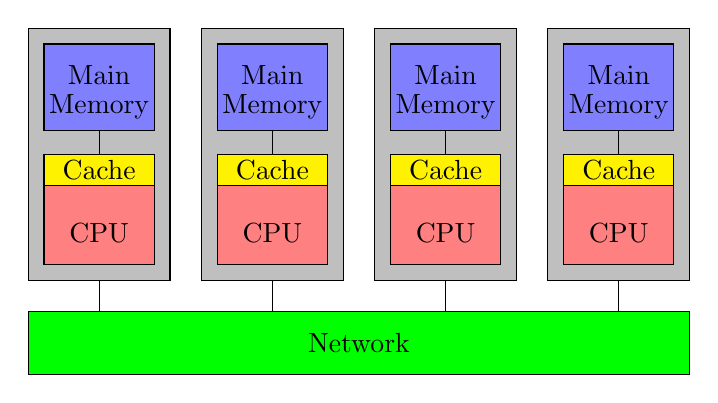
\begin{tikzpicture}[scale=0.4]
        \filldraw[fill=green] (0,-1) rectangle (21,-3);
        \draw (10.5,-2.0) node {Network};
        % First Node
        \filldraw[fill=gray!50!white] (0,0) rectangle (4.5,8);
        \filldraw[fill=blue!50!white] (0.5,4.75) rectangle (4.0,7.5);
        \filldraw[fill=yellow] (0.5,3.0) rectangle (4.0,4,0);
        \filldraw[fill=red!50!white] (0.5,0.5) rectangle (4.0,3.0);
        \draw (2.25,4.0) -- (2.25,4.75);
        \draw (2.25,0) -- (2.25,-1);
        \draw (2.25,6.5) node {Main};
        \draw (2.25,5.5) node {Memory};
        \draw (2.25,1.5) node {CPU};
        \draw (2.25,3.5) node {Cache};
        
        % Second Node
        \filldraw[fill=gray!50!white] (5.5,0) rectangle (10.0,8);
        \filldraw[fill=blue!50!white] (6.0,4.75) rectangle (9.5,7.5);
        \filldraw[fill=yellow] (6.0,3.0) rectangle (9.5,4,0);
        \filldraw[fill=red!50!white] (6.0,0.5) rectangle (9.5,3.0);
        \draw (7.75,4.0) -- (7.75,4.75);
        \draw (7.75,0) -- (7.75,-1);
        \draw (7.75,6.5) node {Main};
        \draw (7.75,5.5) node {Memory};
        \draw (7.75,1.5) node {CPU};
        \draw (7.75,3.5) node {Cache};
        
        % Third Node
        \filldraw[fill=gray!50!white] (11.0,0) rectangle (15.5,8);
        \filldraw[fill=blue!50!white] (11.5,4.75) rectangle (15.0,7.5);
        \filldraw[fill=yellow] (11.5,3.0) rectangle (15.0,4,0);
        \filldraw[fill=red!50!white] (11.5,0.5) rectangle (15.0,3.0);
        \draw (13.25,4.0) -- (13.25,4.75);
        \draw (13.25,0) -- (13.25,-1);
        \draw (13.25,6.5) node {Main};
        \draw (13.25,5.5) node {Memory};
        \draw (13.25,1.5) node {CPU};
        \draw (13.25,3.5) node {Cache};
        
        % Fourth Node
        \filldraw[fill=gray!50!white] (16.5,0) rectangle (21.0,8);
        \filldraw[fill=blue!50!white] (17.0,4.75) rectangle (20.5,7.5);
        \filldraw[fill=yellow] (17.0,3.0) rectangle (20.5,4,0);
        \filldraw[fill=red!50!white] (17.0,0.5) rectangle (20.5,3.0);
        \draw (18.75,4.0) -- (18.75,4.75);
        \draw (18.75,0) -- (18.75,-1);
        \draw (18.75,6.5) node {Main};
        \draw (18.75,5.5) node {Memory};
        \draw (18.75,1.5) node {CPU};
        \draw (18.75,3.5) node {Cache};
      \end{tikzpicture}
    \end{center}
\end{frame}

\begin{frame}
  \frametitle{Shared Memory Model}
%  \begin{columns}
%    \column{6cm}
    \begin{itemize}
      \item All threads can access the global memory space.
      \item Data sharing achieved via writing to/reading from the same memory location
      \item Example
      \begin{itemize}
        \item OpenMP
        \item Pthreads
      \end{itemize}
    \end{itemize}
%    \column{6cm}
    \begin{center}
      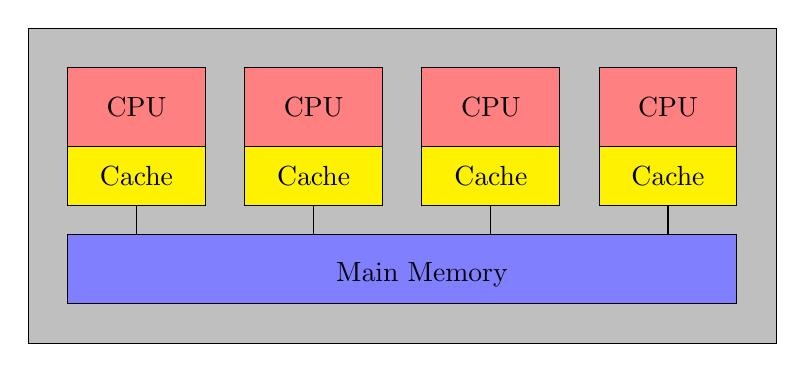
\begin{tikzpicture}[scale=0.5]
        \filldraw[fill=gray!50!white] (0,0) rectangle (19,8);
        \filldraw[fill=blue!50!white] (1,1) rectangle (18,2.75);
        \draw (10,1.75) node {Main Memory};
        % First Core
        \filldraw[fill=yellow] (1,3.5) rectangle (4.5,5.0);
        \draw (2.75,4.25) node {Cache};
        \filldraw[fill=red!50!white] (1,5.0) rectangle (4.5,7.0);
        \draw (2.75,6.0) node {CPU};
        \draw (2.75,3.5) -- (2.75,2.75);
        % Second Core
        \filldraw[fill=yellow] (5.5,3.5) rectangle (9.0,5.0);
        \draw (7.25,4.25) node {Cache};
        \filldraw[fill=red!50!white] (5.5,5.0) rectangle (9.0,7.0);
        \draw (7.25,6.0) node {CPU};
        \draw (7.25,3.5) -- (7.25,2.75);
        % Third Core
        \filldraw[fill=yellow] (10.0,3.5) rectangle (13.5,5.0);
        \draw (11.75,4.25) node {Cache};
        \filldraw[fill=red!50!white] (10.0,5.0) rectangle (13.5,7.0);
        \draw (11.75,6.0) node {CPU};
        \draw (11.75,3.5) -- (11.75,2.75);
        % Fourth Core
        \filldraw[fill=yellow] (14.5,3.5) rectangle (18.0,5.0);
        \draw (16.25,4.25) node {Cache};
        \filldraw[fill=red!50!white] (14.5,5.0) rectangle (18.0,7.0);
        \draw (16.25,6.0) node {CPU};
        \draw (16.25,3.5) -- (16.25,2.75);
      \end{tikzpicture}
%      \includegraphics[width=8cm]{./shared}
    \end{center}
%  \end{columns}
\end{frame}


\begin{frame}
  \frametitle{Clusters of SMP nodes}
  \begin{itemize}
    \item The shared memory model is most commonly represented by Symmetric Multi-Processing (SMP) systems
    \begin{itemize}
      \item Identical processors
      \item Equal access time to memory
    \end{itemize}
    \item Large shared memory systems are rare, clusters of SMP nodes are popular.
  \end{itemize}
%  \begin{columns}
%    \column{13cm}
%    \begin{center}
%      \includegraphics[width=12cm]{./smp-cluster}
%    \end{center}
%  \end{columns}
%\end{frame}

%\begin{frame}
  \begin{center}
    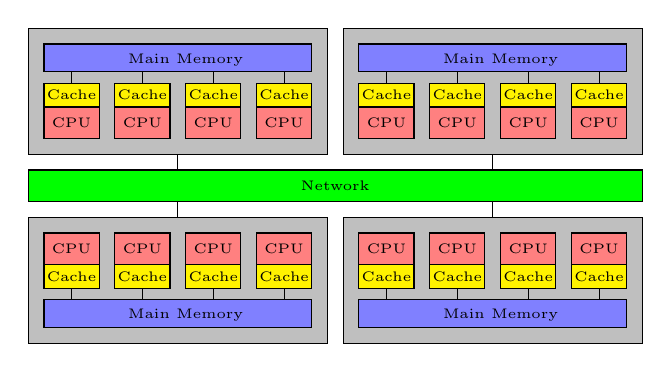
\begin{tikzpicture}[scale=0.2]
      \tikzstyle{every node}=[font=\tiny]
      \filldraw[fill=green] (0,9) rectangle (39,11);
      \draw (19.5,10) node {Network};
      % First Node
      \filldraw[fill=gray!50!white] (0,0) rectangle (19,8);
      \filldraw[fill=blue!50!white] (1,1) rectangle (18,2.75);
      \draw (10,1.75) node {Main Memory};
      % First Core
      \filldraw[fill=yellow] (1,3.5) rectangle (4.5,5.0);
      \draw (2.75,4.25) node {Cache};
      \filldraw[fill=red!50!white] (1,5.0) rectangle (4.5,7.0);
      \draw (2.75,6.0) node {CPU};
      \draw (2.75,3.5) -- (2.75,2.75);
      % Second Core
      \filldraw[fill=yellow] (5.5,3.5) rectangle (9.0,5.0);
      \draw (7.25,4.25) node {Cache};
      \filldraw[fill=red!50!white] (5.5,5.0) rectangle (9.0,7.0);
      \draw (7.25,6.0) node {CPU};
      \draw (7.25,3.5) -- (7.25,2.75);
      % Third Core
      \filldraw[fill=yellow] (10.0,3.5) rectangle (13.5,5.0);
      \draw (11.75,4.25) node {Cache};
      \filldraw[fill=red!50!white] (10.0,5.0) rectangle (13.5,7.0);
      \draw (11.75,6.0) node {CPU};
      \draw (11.75,3.5) -- (11.75,2.75);
      % Fourth Core
      \filldraw[fill=yellow] (14.5,3.5) rectangle (18.0,5.0);
      \draw (16.25,4.25) node {Cache};
      \filldraw[fill=red!50!white] (14.5,5.0) rectangle (18.0,7.0);
      \draw (16.25,6.0) node {CPU};
      \draw (16.25,3.5) -- (16.25,2.75);
      % Connect First Node to Network
      \draw (9.5,8) -- (9.5,9);

      % Second Node
      \filldraw[fill=gray!50!white] (20,0) rectangle (39,8);
      \filldraw[fill=blue!50!white] (21,1) rectangle (38,2.75);
      \draw (30,1.75) node {Main Memory};
      % First Core
      \filldraw[fill=yellow] (21,3.5) rectangle (24.5,5.0);
      \draw (22.75,4.25) node {Cache};
      \filldraw[fill=red!50!white] (21,5.0) rectangle (24.5,7.0);
      \draw (22.75,6.0) node {CPU};
      \draw (22.75,3.5) -- (22.75,2.75);
      % Second Core
      \filldraw[fill=yellow] (25.5,3.5) rectangle (29.0,5.0);
      \draw (27.25,4.25) node {Cache};
      \filldraw[fill=red!50!white] (25.5,5.0) rectangle (29.0,7.0);
      \draw (27.25,6.0) node {CPU};
      \draw (27.25,3.5) -- (27.25,2.75);
      % Third Core
      \filldraw[fill=yellow] (30.0,3.5) rectangle (33.5,5.0);
      \draw (31.75,4.25) node {Cache};
      \filldraw[fill=red!50!white] (30.0,5.0) rectangle (33.5,7.0);
      \draw (31.75,6.0) node {CPU};
      \draw (31.75,3.5) -- (31.75,2.75);
      % Fourth Core
      \filldraw[fill=yellow] (34.5,3.5) rectangle (38.0,5.0);
      \draw (36.25,4.25) node {Cache};
      \filldraw[fill=red!50!white] (34.5,5.0) rectangle (38.0,7.0);
      \draw (36.25,6.0) node {CPU};
      \draw (36.25,3.5) -- (36.25,2.75);
      % Connect Second Node to Network
      \draw (29.5,8) -- (29.5,9);

      % Third Node
      \filldraw[fill=gray!50!white] (0,12) rectangle (19,20);
      \filldraw[fill=blue!50!white] (1,17.25) rectangle (18,19);
      \draw (10,18.0) node {Main Memory};
      % First Core
      \filldraw[fill=yellow] (1,16.5) rectangle (4.5,15.0);
      \draw (2.75,15.75) node {Cache};
      \filldraw[fill=red!50!white] (1,15.0) rectangle (4.5,13.0);
      \draw (2.75,14.0) node {CPU};
      \draw (2.75,16.5) -- (2.75,17.25);
      % Second Core 
      \filldraw[fill=yellow] (5.5,16.5) rectangle (9.0,15.0);
      \draw (7.25,15.75) node {Cache};
      \filldraw[fill=red!50!white] (5.5,15.0) rectangle (9.0,13.0);
      \draw (7.25,14.0) node {CPU};
      \draw (7.25,16.5) -- (7.25,17.25);
      % Third Core 
      \filldraw[fill=yellow] (10.0,16.5) rectangle (13.5,15.0);
      \draw (11.75,15.75) node {Cache};
      \filldraw[fill=red!50!white] (10.0,15.0) rectangle (13.5,13.0);
      \draw (11.75,14.0) node {CPU};
      \draw (11.75,16.5) -- (11.75,17.25);
      % Fourth Core 
      \filldraw[fill=yellow] (14.5,16.5) rectangle (18.0,15.0);
      \draw (16.25,15.75) node {Cache};
      \filldraw[fill=red!50!white] (14.5,15.0) rectangle (18.0,13.0);
      \draw (16.25,14.0) node {CPU};
      \draw (16.25,16.5) -- (16.25,17.25);
      % Connect Third Node to Network
      \draw (9.5,11) -- (9.5,12);

      % Fourth Node
      \filldraw[fill=gray!50!white] (20,12) rectangle (39,20);
      \filldraw[fill=blue!50!white] (21,17.25) rectangle (38,19);
      \draw (30,18.0) node {Main Memory};
      % First Core
      \filldraw[fill=yellow] (21,16.5) rectangle (24.5,15.0);
      \draw (22.75,15.75) node {Cache};
      \filldraw[fill=red!50!white] (21,15.0) rectangle (24.5,13.0);
      \draw (22.75,14.0) node {CPU};
      \draw (22.75,16.5) -- (22.75,17.25);
      % Second Core 
      \filldraw[fill=yellow] (25.5,16.5) rectangle (29.0,15.0);
      \draw (27.25,15.75) node {Cache};
      \filldraw[fill=red!50!white] (25.5,15.0) rectangle (29.0,13.0);
      \draw (27.25,14.0) node {CPU};
      \draw (27.25,16.5) -- (27.25,17.25);
      % Third Core 
      \filldraw[fill=yellow] (30.0,16.5) rectangle (33.5,15.0);
      \draw (31.75,15.75) node {Cache};
      \filldraw[fill=red!50!white] (30.0,15.0) rectangle (33.5,13.0);
      \draw (31.75,14.0) node {CPU};
      \draw (31.75,16.5) -- (31.75,17.25);
      % Fourth Core 
      \filldraw[fill=yellow] (34.5,16.5) rectangle (38.0,15.0);
      \draw (36.25,15.75) node {Cache};
      \filldraw[fill=red!50!white] (34.5,15.0) rectangle (38.0,13.0);
      \draw (36.25,14.0) node {CPU};
      \draw (36.25,16.5) -- (36.25,17.25);
      % Connect Fourth Node to Network
      \draw (29.5,11) -- (29.5,12);
      
    \end{tikzpicture}
  \end{center}
\end{frame}

\begin{frame}
  \frametitle{Shared vs Distributed}
  \vspace{-0.25cm}
%  \begin{columns}
%    \column{5cm}
    \begin{exampleblock}{Shared Memory}
      \begin{itemize}
        \item Pros
        \begin{itemize}
          \item Global address space is user friendly
          \item Data sharing is fast
        \end{itemize}
        \item Cons
        \begin{itemize}
          \item Lack of scalability
          \item Data conflict issues
        \end{itemize}
      \end{itemize}
    \end{exampleblock}
%    \column{5cm}
    \begin{exampleblock}{Distributed Memory}
      \begin{itemize}
        \item Pros
        \begin{itemize}
          \item Memory scalable with number of processors
          \item Easier and cheaper to build
        \end{itemize}
        \item Cons
        \begin{itemize}
          \item Difficult load balancing
          \item Data sharing is slow
        \end{itemize}
      \end{itemize}
    \end{exampleblock}
%  \end{columns}
\end{frame}

\begin{frame}
  \frametitle{Parallelizing Serial Code}
  \begin{exampleblock}{Compiler Flags for Automatic Parallelization}
    \begin{itemize}
      \item \bflub{GCC} -floop-parallelize-all
      \item \bflub{Intel} -parallel
      \item \bflub{NVHPC} -Mconcur
    \end{itemize}
  \end{exampleblock}
  \begin{block}{When to consider using OpenMP?}
    \begin{itemize}
      \item The compiler may not be able to do the parallelization
      \begin{enumerate}
        \item A loop is not parallelized
        \begin{itemize}
          \item The data dependency analysis is not able to determine whether it is safe to parallelize or not
        \end{itemize}
        \item The granularity is not high enough
        \begin{itemize}
          \item The compiler lacks information to parallelize at the highest possible level
        \end{itemize}
      \end{enumerate}
    \end{itemize}
  \end{block}
\end{frame}

\begin{frame}
  \frametitle{OpenMP}
  \begin{block}{}
    \begin{itemize}
      \item OpenMP is an Application Program Interface (API) for thread based parallelism; Supports Fortran, C and C++
      \item Uses a fork-join execution model
      \item OpenMP structures are built with program directives, runtime libraries and environment variables
      \item OpenMP has been the industry standard for shared memory programming since 1997
      \begin{itemize}
        \item Permanent members of the OpenMP Architecture Review Board: AMD, Cray, Fujutsu, HP, IBM, Intel, Microsoft, NEC, PGI, SGI, Sun
      \end{itemize}
      \item OpenMP 4.0 was released in June 2014
    \end{itemize}
  \end{block}
\end{frame}

\begin{frame}
  \frametitle{Goals of OpenMP}
  \vspace{-0.5cm}
  \begin{block}{}
    \begin{itemize}
      \item \bflub{Standardization}
        \begin{itemize}
        \item Provide a standard among a variety of shared memory architectures/platforms
        \item Jointly defined and endorsed by a group of major computer hardware and software vendors
        \end{itemize}
      \item \bflub{Lean and Mean}
        \begin{itemize}
        \item Establish a simple and limited set of directives for programming shared memory machines.
        \item Significant parallelism can be implemented by using just 3 or 4 directives.
        \end{itemize}
      \item \bflub{Ease to use}
      \begin{itemize}
        \item Serial programs can be parallelized by adding compiler directives
        \item Allows for incremental parallelization - a serial program evolves into a parallel program by parallelizing different sections incrementally
      \end{itemize}
      \item \bflub{Portability}
      \begin{itemize}
        \item Standard among many shared memory platforms
        \item Implemented in major compiler suites
      \end{itemize}
    \end{itemize}
  \end{block}
\end{frame}

\begin{frame}
  \frametitle{Fork-Join Execution Model}
  \begin{block}{}
    \begin{itemize}
      \item Parallelism is achieved by generating multiple threads that run in parallel
      \begin{itemize}
        \item A fork \tikz[scale=0.3,baseline=-0.3em]{\filldraw[fill=white] (0.0,0.0) circle (0.5);\draw[draw=black] (0.0,0.0) node {F};} is when a single thread is made into multiple, concurrently executing threads
        \item A join \tikz[scale=0.3,baseline=-0.3em]{\filldraw[fill=white] (0.0,0.0) circle (0.5);\draw[draw=black] (0.0,0.0) node {J};} is when the concurrently executing threads synchronize back into a single thread
      \end{itemize}
      \item OpenMP programs essentially consist of a series of forks and joins.
    \end{itemize}
    \vspace{-0.8cm}
        \begin{center}
      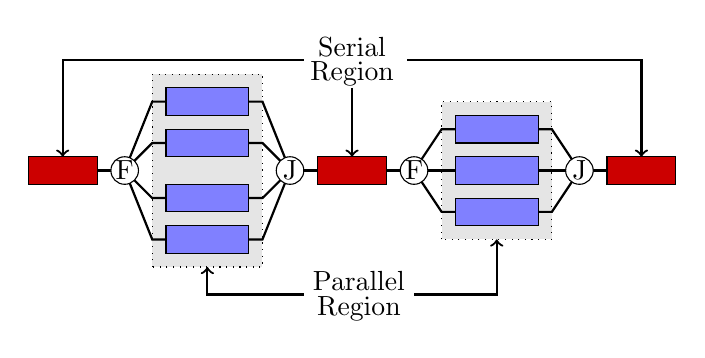
\begin{tikzpicture}[scale=0.35]
        \filldraw[fill=red!80!black] (0,-0.5) rectangle (2.5,0.5);
        \draw[thick] (2.5,0.0) -- (3.5,0.0);
        %Parallel Region 4 threads
        \filldraw[fill=gray!20!white,dotted] (4.5,-3.5) rectangle (8.5,3.5);
        \draw[thick] (3.5,0.0) -- (4.5,2.5) -- (5.0,2.5);
        \draw[thick] (3.5,0.0) -- (4.5,1.0) -- (5.0,1.0);
        \draw[thick] (3.5,0.0) -- (4.5,-1.0) -- (5.0,-1.0);
        \draw[thick] (3.5,0.0) -- (4.5,-2.5) -- (5.0,-2.5);
        \filldraw[fill=blue!50!white] (5.0,2.0) rectangle (8.0,3.0);
        \filldraw[fill=blue!50!white] (5.0,0.5) rectangle (8.0,1.5);
        \filldraw[fill=blue!50!white] (5.0,-0.5) rectangle (8.0,-1.5);
        \filldraw[fill=blue!50!white] (5.0,-2.0) rectangle (8.0,-3.0);
        \draw[thick] (8.0,2.5) -- (8.5,2.5) -- (9.5,0.0);
        \draw[thick] (8.0,1.0) -- (8.5,1.0) -- (9.5,0.0);
        \draw[thick] (8.0,-1.0) -- (8.5,-1.0) -- (9.5,0.0);
        \draw[thick] (8.0,-2.5) -- (8.5,-2.5) -- (9.5,0.0);
        %Serial Region
        \draw[thick] (9.5,0.0) -- (10.5,0.0);
        \filldraw[fill=red!80!black] (10.5,-0.5) rectangle (13.0,0.5);
        \draw[thick] (13.0,0.0) -- (14.0,0.0);
        %Parallel Region 3 threads
        \filldraw[fill=gray!20!white,dotted] (15.0,-2.5) rectangle (19.0,2.5);
        \draw[thick] (14.0,0.0) -- (15.0,1.5) -- (15.5,1.5);
        \draw[thick] (14.0,0.0) -- (15.0,0.0) -- (15.5,0.0);
        \draw[thick] (14.0,0.0) -- (15.0,-1.5) -- (15.5,-1.5);
        \filldraw[fill=blue!50!white] (15.5,1.0) rectangle (18.5,2.0);
        \filldraw[fill=blue!50!white] (15.5,-0.5) rectangle (18.5,0.5);
        \filldraw[fill=blue!50!white] (15.5,-1.0) rectangle (18.5,-2.0);
        \draw[thick] (18.5,1.5) -- (19.0,1.5) -- (20.0,0.0);
        \draw[thick] (18.5,0.0) -- (19.0,0.0) -- (20.0,0.0);
        \draw[thick] (18.5,-1.5) -- (19.0,-1.5) -- (20.0,0.0);
        %Serial Region
        \draw[thick] (20.0,0.0) -- (21.0,0.0);
        \filldraw[fill=red!80!black] (21.0,-0.5) rectangle (23.5,0.5);
        % Add Text
        % Denote Parallel Region
        \draw (12.0,-4.0) node {Parallel} ;
        \draw (12.0,-5.0) node {Region} ;
        \draw[->,thick] (10.0,-4.5) -| (6.5,-3.5);
        \draw[->,thick] (14.0,-4.5) -| (17.0,-2.5);
        % Denote Serial Region
        \draw (11.75,4.5) node {Serial};
        \draw (11.75,3.5) node {Region};
        \draw[->,thick] (11.75,3.0) -- (11.75,0.5);
        \draw[->,thick] (10.0,4.0) -| (1.25,0.5);
        \draw[->,thick] (13.75,4.0) -| (22.25,0.5);
        % Denote Fork and Join Locations
        \filldraw[fill=white] (3.5,0) circle (0.5);
        \filldraw[fill=white] (9.5,0) circle (0.5);
        \filldraw[fill=white] (14.0,0) circle (0.5);
        \filldraw[fill=white] (20.0,0) circle (0.5);
        \draw[draw=black] (3.5,0) node {F};
        \draw[draw=black] (9.5,0) node {J};
        \draw[draw=black] (14.0,0) node {F};
        \draw[draw=black] (20.0,0) node {J};
      \end{tikzpicture}
      \vspace{-0.8cm}
    \end{center}

  \end{block}
\end{frame}

\begin{frame}
  \frametitle{Building Block of OpenMP}
  \begin{exampleblock}{}
    \begin{itemize}
      \item Program directives
        \begin{itemize}
          \item Syntax
            \begin{itemize}
              \item C/C++: \texttt{\#pragma omp <directive> [clause]}
              \item Fortran: \texttt{!\$omp <directive> [clause]}
            \end{itemize}
          \item Parallel regions
          \item Parallel loops
          \item Synchronization
          \item Data Structure
          \item $\cdots$
        \end{itemize}
      \item Runtime library routines
      \item Environment variables
    \end{itemize}
  \end{exampleblock}
\end{frame}

\begin{frame}
  \frametitle{OpenMP Basic Syntax}
  \begin{itemize}
    \item Fortran: case insensitive
    \begin{itemize}
      \item Add: {\color{green!40!black}use} {\color{blue}omp\_lib} or {\color{green!40!black}include} {\color{orange}"omp\_lib.h"}
      \item Usage: {\color{red!90!black}Sentinel directive [clauses]}
      \item Fortran 77
      \begin{itemize}
        \item {\color{red!90!black}Sentinel} could be: {\color{red!90!black}!\$omp, *\$omp, c\$omp} and must begin in first column
      \end{itemize}
      \item Fortran 90/95/2003
      \begin{itemize}
        \item {\color{red!90!black}Sentinel}: {\color{red!90!black}!\$omp}
      \end{itemize}
      \item End of parallel region is signified by the end sentinel statement: {\color{red!90!black}!\$omp end directive [clauses]}
    \end{itemize}
    \item C/C++: case sensitive
    \begin{itemize}
      \item Add {\color{green!40!black}\#include} <{\color{blue}omp.h}>
      \item Usage: {\color{red!90!black}\#pragma omp directive [clauses] newline}
    \end{itemize}
  \end{itemize}
\end{frame}

\begin{frame}{Compiler Directives}
  \begin{itemize}
    \item Parallel Directive
    \begin{itemize}
      \item {\bf\color{red!90!black}parallel}
    \end{itemize}
    \item Worksharing Constructs
    \begin{itemize}
      \item Fortran: {\bf\color{red!90!black}do}, {\bf\color{red!90!black}workshare}
      \item C/C++: {\bf\color{red!90!black}for}
      \item Fortran/C/C++: {\bf\color{red!90!black}sections}
    \end{itemize}
    \item Synchronization
    \begin{itemize}
      \item {\bf\color{red!90!black}master}, {\bf\color{red!90!black}single}, {\bf\color{red!90!black}ordered}, {\bf\color{red!90!black}flush}, {\bf\color{red!90!black}atomic}
    \end{itemize}
  \end{itemize}
\end{frame}

\begin{frame}{Clauses}
  \begin{itemize}
    \item if(scalar\_expression)
    \item private(list), shared(list)
    \item firstprivate(list), lastprivate(list)
    \item reduction(operator:list)
    \item schedule(method[,chunk\_size])
    \item nowait
    \item num\_thread(num)
    \item threadprivate(list), copyin(list)
    \item ordered
    \item more $\cdots$
  \end{itemize}
\end{frame}

\begin{frame}{Runtime Libraries}
  \begin{itemize}
    \item Number of Threads: omp\_\{set,get\}\_num\_threads
    \item Thread ID: omp\_get\_thread\_num
    \item Scheduling: omp\_\{set,get\}\_dynamic
    \item Nested Parallelism: omp\_in\_parallel
    \item Locking: omp\_\{init,set,unset\}\_lock
    \item Wallclock Timer: omp\_get\_wtime
    \item more $\cdots$
  \end{itemize}
\end{frame}

\begin{frame}{Environment Variables}
  \begin{itemize}
    \item OMP\_NUM\_THREADS
    \item OMP\_SCHEDULE
    \item OMP\_STACKSIZE
    \item OMP\_DYNAMIC
    \item OMP\_NESTED
    \item OMP\_WAIT\_POLICY
    \item more $\cdots$
  \end{itemize}
\end{frame}

\begin{frame}{Parallel Directive}
  \begin{itemize}
    \item The {\bf parallel} directive forms a team of threads for parallel execution.
    \item Each thread executes the block of code within the OpenMP Parallel region.
  \end{itemize}
  \vspace{-0.5cm}
  \begin{columns}
    \column{0.45\textwidth}
    \begin{exampleblock}{C}
      \lstinputlisting[language=OmpC]{../slides/code/parprog/src/hello/solution/helloworld.c}
    \end{exampleblock}
    \column{0.45\textwidth}
    \begin{exampleblock}{Fortran}
      \lstinputlisting[language={OmpFortran}]{../slides/code/parprog/src/hello/solution/helloworld.f90}
    \end{exampleblock}
  \end{columns}
\end{frame}

\begin{frame}[fragile]
  \frametitle{Compiling and Running OpenMP programs}
  \vspace{-0.5cm}
  \begin{itemize}
    \item[Compiling:] \lstinline[basicstyle=\normalsize\ttfamily]|compiler options code|
    \item The OpenMP compile flag varies based on the compiler
      \begin{itemize}
        \item[GNU:] \lstinline[basicstyle=\normalsize\ttfamily]|-fopenmp|
        \item[Intel:] \lstinline[basicstyle=\normalsize\ttfamily]|-qopenmp|
        \item[NVHPC:] \lstinline[basicstyle=\normalsize\ttfamily]|-mp|
      \end{itemize}
      \begin{lstlisting}[basicstyle=\small\ttfamily]
[alp514.sol](1032): gfortran -fopenmp -o helloc hello.c
[alp514.sol](1033): ifort -qopenmp -o hellof hello.f90
      \end{lstlisting}
    \item[Running]: Need to specify number of openmp threads to run code on
      \begin{lstlisting}[basicstyle=\small\ttfamily]
[alp514.hawk-b624](1001): OMP_NUM_THREADS=4 ./helloc
Hello world
Hello world
Hello world
Hello world
[alp514.hawk-b624](1002): export OMP_NUM_THREADS=2
[alp514.hawk-b624](1003): ./hellof
 Hello World
 Hello World
      \end{lstlisting}
  \end{itemize}
\end{frame}

\begin{frame}<0>[fragile]
  \frametitle{Compilation and Execution}
  \begin{itemize}
    \item Use any compiler of your choices
      \begin{itemize}
      \item PGI Compiler
        \begin{itemize}
        \item \lstinline[basicstyle=\scriptsize\ttfamily]{module load pgi}
        \item \lstinline[basicstyle=\scriptsize\ttfamily]{pgcc -mp -o hellocmp hello.c}
        \item \lstinline[basicstyle=\scriptsize\ttfamily]{pgfortran -mp -o hellofmp hello.f}
        \end{itemize}
      \item GNU Compiler
        \begin{itemize}
        \item \lstinline[basicstyle=\scriptsize\ttfamily]{module load gcc}
        \item \lstinline[basicstyle=\scriptsize\ttfamily]{gcc -fopenmp -o hellocmp hello.c}
        \item \lstinline[basicstyle=\scriptsize\ttfamily]{gfortran -fopenmp -o hellofmp hello.f}
        \end{itemize}
      \item Intel Compiler
        \begin{itemize}
        \item \lstinline[basicstyle=\scriptsize\ttfamily]{module load intel}
        \item \lstinline[basicstyle=\scriptsize\ttfamily]{icc -qopenmp -o hellocmp hello.c}
        \item \lstinline[basicstyle=\scriptsize\ttfamily]{ifort -qopenmp -o hellofmp hello.f}
        \end{itemize}
      \end{itemize}
  \end{itemize}
  \begin{block}{}
    \begin{lstlisting}[basicstyle=\tiny\ttfamily]
[alp514.sol](752): module load gcc
[alp514.sol](753): gcc -fopenmp -o hellocmp hello.c
[alp514.sol](754): gfortran -fopenmp -o hellofmp hello.f90
[alp514.sol](755): export OMP_NUM_THREADS=4
[alp514.sol](756): srun -p lts -n 1 -c 4 ./hellocmp
Hello world
Hello world
Hello World
Hello World
    \end{lstlisting}
  \end{block}
\end{frame}

\begin{frame}
  \frametitle{Parallel Directive}
  \begin{itemize}
  \item The number of threads in a parallel region is determined by the following factors, in order of precedence:
    \begin{itemize}
    \item Evaluation of the IF clause
    \item Setting of the NUM\_THREADS clause
    \item Use of the omp\_set\_num\_threads() library function
    \item Setting of the OMP\_NUM\_THREADS environment variable
    \item Implementation default
    \end{itemize}
  \item Threads are numbered from 0 (master thread) to N-1
  \end{itemize}
\end{frame}



\begin{frame}[fragile]
  \frametitle{Hello World: C}
  {\scriptsize
  \begin{columns}
    \column{6cm}
    \tikzstyle{na} = [baseline=-.5ex]
    \begin{block}{}
       \begin{tabular}{lc}
        {\color{DarkGreen}\#include <omp.h>} \tikz[na] \node[coordinate] (n1) {}; & \\
        {\color{DarkGreen}\#include <stdio.h>} & \\
        int main () \{ & \\
        \quad {\color{blue}\#pragma omp parallel} & \\
        \quad \{ \tikz[na] \node[coordinate] (n2) {}; & \\
        \quad \quad printf("Hello from thread \%d out of \%d & \\
        \quad \quad\quad threads\textbackslash n'',{\color{red}omp\_get\_thread\_num()} \tikz[na] \node[coordinate] (n3) {}; , & \\
        \quad \quad\quad {\color{red}omp\_get\_num\_threads()}\tikz[na] \node[coordinate] (n4) {}; ); & \\
        \quad \} \tikz[na] \node[coordinate] (n5) {}; & \\
        \quad return 0; & \\
        \} & \\
      \end{tabular}
    \end{block}
    \column{4cm}
    \vspace{-0.5cm}
    \begin{itemize}
      \item[] \tikz[baseline]{\node[fill=blue!20,anchor=base] (t1) {OpenMP include file}; } 
      \item[]
      \item[] \tikz[baseline]{\node[fill=blue!20,anchor=base] (t2) {Parallel region starts here};  } 
      \item[]
      \item[] \tikz[baseline]{\node[fill=blue!20,anchor=base] (t3) {Runtime library functions};  }
      \item[]
      \item[] \tikz[baseline]{\node[fill=blue!20,anchor=base] (t4) {Parallel region ends here};  }
    \end{itemize}
    \begin{tikzpicture}[overlay]
        \path[->] (t1) edge (n1);
        \path[->] (t2) edge (n2);
        \path[->] (t3) edge (n3);
        \path[->] (t3) edge (n4);
        \path[->] (t4) edge (n5);
    \end{tikzpicture}
  \end{columns}
  \begin{columns}
    \column{6cm}
    \begin{exampleblock}{}
    \begin{Verbatim}
Hello from thread 0 out of 4 threads
Hello from thread 3 out of 4 threads
Hello from thread 1 out of 4 threads
Hello from thread 2 out of 4 threads
    \end{Verbatim}
    \end{exampleblock}
  \end{columns}
  }
\end{frame}

{\scriptsize
\begin{frame}[fragile]
  \frametitle{Hello World: Fortran}
  \begin{columns}
    \column{6cm}
    \tikzstyle{na} = [baseline=-.5ex]
    \begin{block}{}
       \begin{tabular}{lc}
         program hello & \\
         \\
        \quad implicit none & \\
        \quad integer :: omp\_get\_thread\_num, omp\_get\_num\_threads & \\
        \\
        \quad {\color{blue} !\$omp parallel} \tikz[na] \node[coordinate] (n2) {}; & \\
        \\
        \quad print '(a,i3,a,i3,a)', 'Hello from thread', & \\
        \quad\quad {\color{red}omp\_get\_thread\_num()} \tikz[na] \node[coordinate] (n3) {}; , \& & \\
        \quad\quad ' out of ' {\color{red}omp\_get\_num\_threads()}\tikz[na] \node[coordinate] (n4) {};,' threads' & \\
        \\
        \quad {\color{blue} !\$omp end parallel} \tikz[na] \node[coordinate] (n5) {}; & \\
        end program hello & \\ 
      \end{tabular}
    \end{block}
    \column{4cm}
%    \vspace{-0.5cm}
    \begin{itemize}
 %     \item[] \tikz[baseline]{\node[fill=blue!20,anchor=base] (t1) {OpenMP include file}; } 
 %     \item[]
      \item[]
      \item[] \tikz[baseline]{\node[fill=blue!20,anchor=base] (t2) {Parallel region starts here};  } 
      \item[]
      \item[]
      \item[] \tikz[baseline]{\node[fill=blue!20,anchor=base] (t3) {Runtime library functions};  }
      \item[]
      \item[] \tikz[baseline]{\node[fill=blue!20,anchor=base] (t4) {Parallel region ends here};  }
    \end{itemize}
    \begin{tikzpicture}[overlay]
%        \path[->] (t1) edge (n1);
        \path[->] (t2) edge  (n2);
        \path[->] (t3) edge [bend right] (n3);
        \path[->] (t3) edge [bend left] (n4);
        \path[->] (t4) edge [bend left] (n5);
    \end{tikzpicture}
  \end{columns}
  \begin{columns}
    \column{8cm}
    \begin{exampleblock}{}
      \begin{Verbatim}
Hello from thread  0 out of   4 threads
Hello from thread  2 out of   4 threads
Hello from thread  1 out of   4 threads
Hello from thread  3 out of   4 threads
      \end{Verbatim}
    \end{exampleblock}
  \end{columns}
\end{frame}
}
\footnotesize

\begin{frame}[fragile]
  \frametitle{Exercise 1: Hello World}
  \begin{itemize}
    \item Write a ``hello world'' program with OpenMP where
      \begin{enumerate}
        \item If the thread id is odd, then print a message "Hello world from thread x, I'm odd!''
        \item If the thread id is even, then print a message "Hello world from thread x, I'm even!''
      \end{enumerate}
    \item Running the example interactively, say you compiled the code as helloc
	  \begin{lstlisting}[basicstyle=\footnotesize\ttfamily]
srun -p hawkgpu -n 6 -t 30 -A hpc2021_prog_083121 --reservation=lts_165 --pty /bin/bash
export OMP_NUM_THREADS=6
./helloc
           \end{lstlisting}
     \item Run from the head node: 
       \begin{lstlisting}[basicstyle=\footnotesize\ttfamily]
export OMP_NUM_THREADS=6
srun -p hawkgpu -n 6 -t 30 -A hpc2021_prog_083121 --reservation=lts_165 ./helloc
       \end{lstlisting}
     \item Alternate way to run from the head node: 
       \begin{lstlisting}[basicstyle=\footnotesize\ttfamily]
srun -p hawkgpu -n 1 -c 6 -t 30 -A hpc2021_prog_083121 --reservation=lts_165 --export=OMP_NUM_THREADS=6  ./helloc
       \end{lstlisting}
  \end{itemize}
%  \begin{columns}
%    \column{0.45\textwidth}
%    \begin{block}{C}
%      \lstinputlisting[language=OmpC]{../slides/code/parprog/src/hello/exercise/hello.c}
%    \end{block}
%    \column{0.45\textwidth}
%    \begin{block}{Fortran}
%      \lstinputlisting[language=OmpFortran]{../slides/code/parprog/src/hello/exercise/hello.f90}
%    \end{block}
%  \end{columns}
\end{frame}

\begin{frame}[fragile]
  \frametitle{Solution}
  \begin{columns}
    \column{0.45\textwidth}
    \begin{exampleblock}{C/C++}
      \lstinputlisting[language=OmpC]{../slides/code/parprog/src/hello/solution/hello.c}
    \end{exampleblock}
    \begin{block}{}
      {\fontsize{4}{5}\selectfont
        \begin{Verbatim}
[alp514.hawk-b624](1003): icc -o hello -qopenmp hello.c
[alp514.hawk-b624](1004): icc -o helloc -qopenmp hello.c
[alp514.hawk-b624](1005): OMP_NUM_THREADS=4 ./helloc
Hello world from thread 0, I am even
Hello world from thread 2, I am even
Hello world from thread 1, I am odd
Hello world from thread 3, I am odd
        \end{Verbatim}
      }
    \end{block}
    \column{0.45\textwidth}
    \begin{exampleblock}{Fortran}
      \lstinputlisting[language={OmpFortran}]{../slides/code/parprog/src/hello/solution/hello.f90}
    \end{exampleblock}
    \begin{block}{}
      {\fontsize{4}{5}\selectfont
        \begin{Verbatim}
[alp514.hawk-b624](1006): ifort -qopenmp -o hellof hello.f90
[alp514.hawk-b624](1007): export OMP_NUM_THREADS=4
[alp514.hawk-b624](1008): ./hellof
 Hello from thread           0 , I am even!
 Hello from thread           2 , I am even!
 Hello from thread           1 , I am odd!
 Hello from thread           3 , I am odd!
        \end{Verbatim}
      }
    \end{block}
  \end{columns}
\end{frame}

\begin{frame}
  \frametitle{Work Sharing}
  \begin{itemize}
    \item We need to share work among threads to achieve parallelism
  \begin{columns}
    \column{0.33\textwidth}
    \begin{block}{Loops}
      \centering{
        {\scriptsize
          \texttt{!\$omp do}
          
          \texttt{\#pragma omp for}
          \\
        }
        \includegraphics[width=0.5\textwidth]{../slides/image/parprog/work_share1}
      }
    \end{block}
    \column{0.33\textwidth}
    \begin{block}{Sections}
      \centering{
        {\scriptsize
          \texttt{!\$omp sections} 
          
          \texttt{\#pragma sections} 
          \\
        }
        \includegraphics[width=0.5\textwidth]{../slides/image/parprog/work_share2}
      }
    \end{block}
    \column{0.33\textwidth}
    \begin{block}{Single}
      \centering{
        {\scriptsize
          \texttt{!\$omp single}
          
          \texttt{\#pragma omp single}
          \\
        }
        \includegraphics[width=0.5\textwidth]{../slides/image/parprog/work_share3}
      }
    \end{block}
  \end{columns}
    \item The parallel and work sharing directive can be combined as
    \begin{itemize}
      \item \texttt{!\$omp parallel do}
      \item \texttt{\#pragma omp parallel sections}
    \end{itemize}
  \end{itemize}
\end{frame}

\begin{frame}[fragile]
  \frametitle{Example: Parallel Loops}
  \begin{columns}
    \column{0.45\textwidth}
    \begin{exampleblock}{C/C++}
        \begin{lstlisting}[basicstyle=\footnotesize\ttfamily,language=OmpC]
#include <omp.h>

int main() {
  int i = 0, n = 100, a[100];
  #pragma omp parallel for
  for (i = 0; i < n ; i++) {
    a[i] = (i+1) * (i+2) ;
  }
}
        \end{lstlisting}
     \end{exampleblock}
    \column{0.45\textwidth}
    \begin{exampleblock}{Fortran}
        \begin{lstlisting}[basicstyle=\footnotesize\ttfamily,language=OmpFortran]
program paralleldo

  implicit none
  integer :: i, n, a(100)
  
  i = 0
  n = 100
  !$omp parallel 
  !$omp do
  do i = 1, n
     a(i) = i * (i+1)
  end do
  !$omp end do
  !$omp end parallel
end program paralleldo
        \end{lstlisting}
    \end{exampleblock}
  \end{columns}
\end{frame}

\begin{frame}[allowframebreaks]
  \frametitle{Load Balancing}
  \begin{itemize}
    \item OpenMP provides different methods to divide iterations among threads, indicated by the \texttt{schedule} clause
    \begin{itemize}
      \item Syntax: \texttt{schedule (<method>, [chunk size])}
    \end{itemize}
    \item Methods include
    \begin{itemize}
      \item \texttt{Static}: the default schedule; divide interations into chunks according to \texttt{size}, then distribute chunks to each thread in a round-robin manner.
      \item \texttt{Dynamic}: each thread grabs a chunk of iterations, then requests another chunk upon completion of the current one, until all iterations are executed.
      \item \texttt{Guided}: similar to \texttt{Dynamic}; the only difference is that the chunk size starts large and shrinks to \texttt{size} eventually.
    \end{itemize}
  \end{itemize}

  \begin{block}{4 threads, 100 iterations}
    \begin{tabular}{ccccc}
      \multirow{2}{*}{Schedule}& \multicolumn{4}{c}{Iterations mapped onto thread}\\
      & 0 & 1 & 2 & 3 \\
      \hline
      \texttt{Static} & 1-25 & 26-50 & 51-75 & 76-100 \\
      \texttt{Static,20} & 1-20, 81-100 & 21-40 & 41-60 & 61-80 \\
      \texttt{Dynamic} & $1,\cdots$ & $2,\cdots$ & $3,\cdots$ & $4,\cdots$ \\
      \texttt{Dynamic,10} & $1-10,\cdots$ & $11-20,\cdots$ & $21-30,\cdots$ & $31-40,\cdots$ \\
      \hline\\
    \end{tabular}
  \end{block}

  \begin{block}{}
    \begin{center}
      \begin{tabular}{cl}
        Schedule & When to Use \\
        \hline\\
        \multirow{3}{*}{\texttt{Static}} & Even and predictable workload per iteration; \\
        & scheduling may be done at compilation time,\\ 
        & least work at runtime.\\
        \\
        \multirow{2}{*}{\texttt{Dynamic}} & Highly variable and unpredictable workload \\
        & per iteration; most work at runtime \\
        \\
        \multirow{3}{*}{\texttt{Guided}} & Special case of \texttt{dynamic} scheduling; \\
        & compromise between load balancing and \\
        & scheduling overhead at runtime \\
      \end{tabular}
    \end{center}
  \end{block}
\end{frame}

\begin{frame}[fragile]
  \frametitle{Work Sharing: Sections}
  \begin{itemize}
    \item Gives a different block to each thread
  \end{itemize}
  \begin{columns}
    \column{0.45\textwidth}
    \begin{exampleblock}{C/C++}
      \lstinputlisting[basicstyle=\footnotesize\ttfamily,language=OmpC,firstline=10,lastline=21]{../slides/code/parprog/src/tmp.c}
    \end{exampleblock}
    \column{0.45\textwidth}
    \begin{exampleblock}{Fortran}
      \lstinputlisting[basicstyle=\footnotesize\ttfamily,language=OmpFortran,firstline=14,lastline=23]{../slides/code/parprog/src/tmp.f90}
    \end{exampleblock}
  \end{columns}
\end{frame}


\begin{frame}
  \frametitle{Scope of variables}
  \begin{itemize}
    \item \texttt{Shared(list)}
    \begin{itemize}
      \item Specifies the variables that are shared among all threads
    \end{itemize}
    \item \texttt{Private(list)}
    \begin{itemize}
      \item Creates a local copy of the specified variables for each thread
      \item the value is uninitialized!
    \end{itemize}
    \item \texttt{Default(shared|private|none)}
    \begin{itemize}
      \item Defines the default scope of variables
      \item \textbf{C/C++ API does not have \texttt{default(private)}}
    \end{itemize}
    \item Most variables are shared by default
    \begin{itemize}
      \item A few exceptions: iteration variables; stack variables in subroutines; automatic variables within a statement block.
    \end{itemize}
  \end{itemize}
\end{frame}

\begin{frame}{Exercise: SAXPY}
  \begin{itemize}
    \item SAXPY is a common operation in computations with vector processors included as part of the BLAS routines
    \item[] $y\leftarrow \alpha x + y$
    \item SAXPY is a combination of scalar multiplication and vector addition
    \item Parallelize the code in the \texttt{exercise/saxpy} folder
    \item Calculate the speedup with respect to serial code.
  \end{itemize}
%  \vspace{-0.5cm}
%  \begin{columns}
%    \column{0.45\textwidth}
%    \begin{block}{C}
%      \lstinputlisting[basicstyle=\fontsize{3.5}{4}\selectfont\ttfamily,language=OmpC]{../slides/code/parprog/src/saxpy/solution/saxpy.c}
%    \end{block}
%    \column{0.45\textwidth}
%    \begin{block}{Fortran}
%      \lstinputlisting[basicstyle=\fontsize{3.5}{4}\selectfont\ttfamily,language=OmpFortran]{../slides/code/parprog/src/saxpy/solution/saxpy.f90}
%    \end{block}
%  \end{columns}
\end{frame}

\begin{frame}<0>{Solution: SAXPY}
  \vspace{-0.5cm}
  \begin{columns}
    \column{0.45\textwidth}
    \begin{exampleblock}{C}
      \lstinputlisting[basicstyle=\fontsize{3.5}{4}\ttfamily,language=OmpC]{../slides/code/parprog/src/saxpy/solution/saxpy_omp.c}
    \end{exampleblock}
    \column{0.45\textwidth}
    \begin{exampleblock}{Fortran}
      \lstinputlisting[basicstyle=\fontsize{3.5}{4}\selectfont\ttfamily,language=OmpFortran]{../slides/code/parprog/src/saxpy/solution/saxpy_omp.f90}
    \end{exampleblock}
  \end{columns}
  \begin{columns}
    \column{0.8\textwidth}
    {
      \begin{exampleblock}{}
        \begin{tabular}{|b|b|b|b|}
          \hline
          \rowcolor{lublue}Language & Serial & OpenMP (6 Threads) & SpeedUp \\
          \hline
          C & 0.512128 & 0.087660 & 5.84 \\ \hline
          Fortran & 0.504534 & 0.100535 & 5.02 \\
          \hline
        \end{tabular}
      \end{exampleblock}
    }
  \end{columns}
\end{frame}

\begin{frame}{SAXPY Timing}
  \begin{exampleblock}{}
    \begin{center}
      \begin{tabular}{|b|b|b|b|b|}
        \hline
        \rowcolor{lublue}Threads & \multicolumn{2}{b|}{C} & \multicolumn{2}{b|}{Fortran} \\
        \cline{2-5}
        \rowcolor{lublue}& Timing (s) & Speed Up & Timing (s) & Speed Up \\
        \hline
        1 & 0.513491  &  1.00  & 0.504534  &   1.00 \\
        2 & 0.264634  &  1.94  & 0.300650  &   1.68 \\
        3 & 0.177902  &  2.89  & 0.234661  &   2.15 \\
        4 & 0.135248  &  3.80  & 0.150547  &   3.35 \\
        5 & 0.109646  &  4.68  & 0.120734  &   4.18 \\
        6 & 0.087660  &  5.86  & 0.100535  &   5.02 \\
        12 & 0.056454 &  9.10  & 0.050300  &  10.03 \\
        24 & 0.048442 & 10.60  & 0.026623  &  18.95 \\
        48 & 0.026348 & 19.49  & 0.025263  &  19.97 \\
        \hline
      \end{tabular}
    \end{center}
    \end{exampleblock}
\end{frame}

\begin{frame}[fragile]
  \frametitle{Pitfalls: False Sharing}
  \begin{itemize}
    \item Array elements that are in the same cache line can lead to false sharing.
    \begin{itemize}
      \item The system handles cache coherence on a cache line basis, not on a byte or word basis.
      \item Each update of a single element could invalidate the entire cache line.
    \end{itemize}
  \end{itemize}
  \begin{columns}
    \column{0.45\textwidth}
    \begin{center}
      \includegraphics[width=0.75\textwidth]{../slides/image/parprog/falsesharing}
    \end{center}
    \column{0.45\textwidth}
    \begin{exampleblock}{}
      \lstinputlisting[basicstyle=\footnotesize\ttfamily,language=OmpFortran,firstline=51,lastline=57]{../slides/code/parprog/src/tmp.f90}
    \end{exampleblock}
  \end{columns}
\end{frame}

\begin{frame}
  \frametitle{Pitfalls: Race Condition}
  \begin{itemize}
    \item Multiple threads try to write to the same memory location at the same time.
    \begin{itemize}
      \item Indeterministic results
    \end{itemize}
    \item Inappropriate scope of varibale can cause indeterministic results too.
    \item When having indeterministic results, set the number of threads to 1 to check
    \begin{itemize}
      \item If problem persists: scope problem
      \item If problem is solved: race condition
    \end{itemize}
  \end{itemize}
  \begin{columns}
    \column{0.5\textwidth}
    \vspace{-0.5cm}
    \begin{exampleblock}{}
      \lstinputlisting[basicstyle=\footnotesize\ttfamily,language=OmpFortran,firstline=59,lastline=65]{../slides/code/parprog/src/tmp.f90}
    \end{exampleblock}
  \end{columns}
\end{frame}

\begin{frame}
  \frametitle{Synchronization: Barrier}
  \begin{itemize}
    \item ``Stop sign'' where every thread waits until all threads arrive.
    \item Purpose: protect access to shared data.
    \item Syntax:
    \begin{itemize}
      \item Fortran: \texttt{!\$omp barrier}
      \item C/C++: \texttt{\#pragma omp barrier}
    \end{itemize}
    \item A barrier is implied at the end of every parallel region
    \begin{itemize}
      \item Use the \texttt{nowait} clause to turn it off
    \end{itemize}
    \item Synchronizations are costly so their usage should be minimized.
  \end{itemize}
\end{frame}

\begin{frame}
  \frametitle{Synchronization: Crtitical and Atomic}
%  \begin{itemize}
%    \item Critical: Only one thread at a time can enter a \texttt{critical} region 
%  \end{itemize}
  \begin{columns}
    \column{0.5\textwidth}
    \begin{exampleblock}{Critical}
      Only one thread at a time can enter a \texttt{critical} region
      \lstinputlisting[basicstyle=\footnotesize\ttfamily,language=OmpFortran,firstline=67,lastline=73]{../slides/code/parprog/src/tmp.f90}
    \end{exampleblock}
%  \end{columns}
%  \begin{itemize}
%    \item Atomic: Only one thread at a time can update a memory location 
%  \end{itemize}
%  \begin{columns}
    \column{0.5\textwidth}
    \begin{exampleblock}{Atomic}
      Only one thread at a time can update a memory location
      \lstinputlisting[basicstyle=\footnotesize\ttfamily,language=OmpFortran,firstline=75,lastline=81]{../slides/code/parprog/src/tmp.f90}
    \end{exampleblock}  
  \end{columns}
\end{frame}

\begin{frame}[fragile]
  \frametitle{Private Variables}
  \begin{itemize}
    \item Not initialized at the beginning of parallel region.
    \item After parallel region
    \begin{itemize}
      \item Not defined in OpenMP 2.x
      \item 0 in OpenMP 3.x
    \end{itemize}
  \end{itemize}
  \def\firstnode{\tikz[remember picture,baseline=-0.5mm] \node (n1) {tmp};}  
  \def\secondnode{\tikz[remember picture,baseline=-0.5mm] \node (n2) {tmp};} 
  \begin{exampleblock}{}
    \centering{\hspace{1.45cm}\tikz[remember picture] \node[coordinate,fill=blue!20,rectangle] (t1) {tmp not initialized here};}
    {\scriptsize
      \begin{Verbatim}[commandchars=\|\§\! ]
        void wrong()
        {
          int tmp = 0;
          #pragma omp for private(|firstnode)
          for (int j = 0; j < 100; ++j)
          tmp += j
          printf("%d\n", |secondnode)
        }
      \end{Verbatim}
    }
    \vspace{0.2cm}
    {\hspace{-2.3cm}
      \tikz[remember picture] \node[coordinate,fill=blue!20,rectangle] (t2) {OpenMP 2.5: tmp undefined};
      \tikz[remember picture] \node[coordinate,fill=blue!20,rectangle] (t3) {OpenMP 3.0: tmp is 0};
}
    \begin{tikzpicture}[remember picture,overlay]
      \path[->] (t1) edge (n1);
      \path[->] (t2) edge (n2);
      \path[->] (t3) edge (n2);
    \end{tikzpicture}
  \end{exampleblock}
\end{frame}

\begin{frame}[fragile]
  \frametitle{Special Cases of Private}
  \begin{itemize}
    \item Firstprivate
    \begin{itemize}
      \item Initialize each private copy with the corresponding value from the master thread
    \end{itemize}
    \item Lastprivate
    \begin{itemize}
      \item Allows the value of a private variable to be passed to the shared variable outside the parallel region
    \end{itemize}
  \end{itemize}
  \def\firstnode{\tikz[remember picture,baseline=-0.5mm] \node (n1) {tmp};}  
  \def\secondnode{\tikz[remember picture,baseline=-0.5mm] \node (n2) {tmp};} 
  \begin{exampleblock}{}
    \centering{\hspace{0.3cm}\tikz[remember picture] \node[coordinate,fill=blue!20,rectangle] (t1) {tmp initialized as 0};}
    {\scriptsize
      \begin{Verbatim} [commandchars=\|\§\! ]
void wrong()
{
  int tmp = 0;
  #pragma omp for firstprivate(|firstnode) lastprivate(tmp)
  for (int j = 0; j < 100; ++j)
    tmp += j
  printf("%d\n", |secondnode)
}
      \end{Verbatim}
    }
    \vspace{0.2cm}
    {\hspace{-4.3cm}\tikz[remember picture] \node[coordinate,fill=blue!20,rectangle] (t2) {The value of tmp is the value when j=99};}
    \begin{tikzpicture}[remember picture,overlay]
      \path[->] (t1) edge (n1);
      \path[->] (t2) edge (n2);
    \end{tikzpicture}
  \end{exampleblock}
\end{frame}

\begin{frame}
  \frametitle{Exercise: Calculate pi by Numerical Integration}
  \begin{columns}
    \column{5cm}
    \vspace{-0.5cm}
    \begin{itemize}
      \item We know that
      \begin{align*}
        \int^1_0 \dfrac{4.0}{(1+x^2)}\, dx = \pi
      \end{align*}
      \item So numerically, we can approxiate pi as the sum of a number of rectangles
      \begin{align*}
        \sum^N_{i=0}\,F(x_i)\Delta x \approx \pi
      \end{align*}
      \item[] {\fontsize{4}{5}{ Meadows et al, A ``hands-on'' introduction to OpenMP, SC09 }}
      \item Parallelize the code in the \texttt{exercise/calc\_pi} folder
    \end{itemize}
    \column{5cm}
    \begin{center}
      \includegraphics[width=4cm]{../slides/image/parprog/pi}
    \end{center}
  \end{columns}
\end{frame}

\begin{frame}<0>[fragile]
  \frametitle{Exercise: Rewrite for OpenMP parallelization}
  \begin{columns}
    \column{0.45\textwidth}
    \begin{exampleblock}{C/C++}
      \lstinputlisting[basicstyle=\fontsize{5}{6}\selectfont\ttfamily,language=C]{../slides/code/parprog/src/calc_pi/exercise/pi_serial.c}
    \end{exampleblock}
    \column{0.45\textwidth}
    \begin{exampleblock}{Fortran}
      \lstinputlisting[basicstyle=\fontsize{5}{6}\selectfont\ttfamily,language={[90]Fortran}]{../slides/code/parprog/src/calc_pi/exercise/pi_serial.f90}
    \end{exampleblock}
  \end{columns}
\end{frame}

\begin{frame}<0>[fragile,allowframebreaks]
  \frametitle{Solution (Very Slow)}
  \begin{columns}
    \column{0.45\textwidth}
    \vspace{-0.5cm}
    \begin{exampleblock}{C/C++}
      \lstinputlisting[basicstyle=\fontsize{5}{6}\selectfont\ttfamily,language=OmpC]{../slides/code/parprog/src/calc_pi/solution/pi_omp1.c}
    \end{exampleblock}
    \column{0.45\textwidth}
    \vspace{-0.5cm}
    \begin{exampleblock}{Fortran}
      \lstinputlisting[basicstyle=\fontsize{5}{6}\ttfamily,language=OmpFortran]{../slides/code/parprog/src/calc_pi/solution/pi_omp1.f90}
    \end{exampleblock}
  \end{columns}
  \begin{block}{}
    {\tiny
      \begin{verbatim}
altair:openmp apacheco$ gcc pi_serial.c -o pic
altair:openmp apacheco$ gcc -fopenmp pi_omp1.c -o pic_omp
altair:openmp apacheco$ gfortran pi_serial.f90 -o pif
altair:openmp apacheco$ gfortran -fopenmp pi_omp1.f90 -o pif_omp
altair:solution apacheco$ echo ``Serial C Code''; ./pic
Serial C Code
pi = 3.141592653590426
time to compute = 1.72441 seconds
altair:solution apacheco$ echo ``OMP C Code with Atomic''; ./pic_omp
OMP C Code with Atomic
pi = 3.141592653590195
time to compute = 6.10142 seconds
altair:solution apacheco$ echo ``Serial F90 Code''; ./pif
Serial F90 Code
pi = 3.141592673590427
time to compute = 0.988196 seconds
altair:solution apacheco$ echo ``OMP F90 Code with Atomic''; ./pif_omp
OMP F90 Code with Atomic
pi = 3.141592673590174
time to compute = 7.368610 seconds
      \end{verbatim}
    }
  \end{block}
  \begin{itemize}
    \item What is the value of pi if you did not have the \textit{atomic} directive?
  \end{itemize}
\end{frame}

\begin{frame}
  \frametitle{Reduction}
  \begin{itemize}
    \item The \texttt{reduction} clause allows accumulative operations on the value of variables.
    \item Syntax: \texttt{reduction (operator:variable list)}
    \item A private copy of each variable which appears in \texttt{reduction} is created as if the \texttt{private} clause is specified.
    \item Operators
    \begin{enumerate}
      \item Arithmetic
      \item Bitwise
      \item Logical
    \end{enumerate}
  \end{itemize}
\end{frame}

\begin{frame}[fragile]
  \frametitle{Example: Reduction}
  \begin{columns}
    \column{0.45\textwidth}
    \begin{exampleblock}{C/C++}
      {\tiny
        \begin{lstlisting}[basicstyle=\footnotesize\ttfamily,language=OmpC]
#include <omp.h>
int main() {
  int i, n = 100, sum , a[100], b[100];
  for (i = 0; i < n; i++) {
    a[i] = i;
    b[i] = 1;
  }
  sum = 0;
#pragma omp parallel for reduction(+:sum)
  for (i = 0; i < n ; i++) {
    sum += a[i] * b[i];
  }
}
        \end{lstlisting}
      }
    \end{exampleblock}
    \column{0.45\textwidth}
    \begin{exampleblock}{Fortran}
      {\tiny
        \begin{lstlisting}[basicstyle=\footnotesize\ttfamily,language=OmpFortran]
program reduction
  
  implicit none
  integer :: i, n, sum , a(100), b(100)

  n = 100 ; b = 1; sum = 0
  do i = 1 , n
     a(i) = i
  end do
  !$omp parallel do reduction(+:sum)
  do i = 1, n
     sum = sum + a(i) * b(i)
  end do
  !$omp end parallel do

end program reduction
        \end{lstlisting}
      }
    \end{exampleblock}
  \end{columns}
\end{frame}

\begin{frame}
  \frametitle{Exercise 3: pi calculation with reduction}
  \begin{itemize}
    \item Redo exercise 2 with reduction
  \end{itemize}
\end{frame}

\begin{frame}<0>[fragile,allowframebreaks]
  \frametitle{Solution: pi calculation with reduction}
  \begin{columns}
    \column{5cm}
    \begin{exampleblock}{C }
      \lstinputlisting[basicstyle=\fontsize{5}{6}\selectfont\ttfamily,language=OmpC]{../slides/code/parprog/src/calc_pi/solution/pi_omp.c}
    \end{exampleblock}
    \column{5cm}
    \begin{exampleblock}{Fortran}
      \lstinputlisting[basicstyle=\fontsize{5}{6}\ttfamily,language=OmpFortran]{../slides/code/parprog/src/calc_pi/solution/pi_omp.f90}
    \end{exampleblock}
  \end{columns}
  \begin{block}{}
    {\tiny
      \begin{verbatim}
altair:openmp apacheco$ gcc -fopenmp pi_omp.c -o pic_ompr
altair:openmp apacheco$ gfortran -fopenmp pi_omp.f90 -o pif_ompr
altair:solution apacheco$ echo ``Serial C Code''; ./pic
Serial C Code
pi = 3.141592653590426
time to compute = 1.72441 seconds
altair:solution apacheco$ echo ``OMP C Code with Atomic''; ./pic_omp
OMP C Code with Atomic
pi = 3.141592653590195
time to compute = 6.10142 seconds
altair:solution apacheco$ echo ``OMP C Code with Reduction''; ./pic_ompr
OMP C Code with Reduction
pi = 3.141592653589683
time to compute = 0.48712 seconds
altair:solution apacheco$ echo ``Serial F90 Code''; ./pif
Serial F90 Code
pi = 3.141592673590427
time to compute = 0.988196 seconds
altair:solution apacheco$ echo ``OMP F90 Code with Atomic''; ./pif_omp
OMP F90 Code with Atomic
pi = 3.141592673590174
time to compute = 7.368610 seconds
altair:solution apacheco$ echo ``OMP F90 Code with Reduction''; ./pif_ompr
OMP F90 Code with Reduction
pi = 3.141592673589683
time to compute = 0.400939 seconds
      \end{verbatim}
    }
  \end{block}
\end{frame}

\begin{frame}{Exercise: Matrix Multiplication}
  \begin{itemize}
    \item Most Computational code involve matrix operations such as matrix multiplication.
    \item Consider a matrix {\bf C} of two matrices {\bf A} and {\bf B}:
    \item[] Element {\it i,j} of {\bf C} is the dot product of the $i^{th}$ row of {\bf A} and $j^{th}$ column of {\bf B}
      \begin{center}
        \includegraphics[width=0.5\textwidth]{../slides/image/parprog/matmul}
      \end{center}
    \item Parallelize the code in the \texttt{exercise/matmul} folder
    \item Calculate the speedup with respect to serial code.
  \end{itemize}
%  \framebreak
%  \begin{columns}
%    \column{0.45\textwidth}
%    \vspace{-1cm}
%    \begin{block}{C}
%      \lstinputlisting[basicstyle=\fontsize{3.5}{3.5}\selectfont\ttfamily,language=OmpC]{../slides/code/parprog/src/matmul/exercise/matmul.c}
%    \end{block}
%    \column{0.45\textwidth}
%    \vspace{-1cm}
%    \begin{block}{Fortran}
%      \lstinputlisting[basicstyle=\fontsize{3.5}{3.5}\selectfont\ttfamily,language=OmpFortran]{../slides/code/parprog/src/matmul/exercise/matmul.f90}
%    \end{block}
%  \end{columns}
\end{frame}

\begin{frame}<0>{MATMUL Timing}
  \begin{exampleblock}{}
    \begin{center}
      \begin{tabular}{|b|b|b|b|b|}
        \hline
        \rowcolor{lublue}Threads & \multicolumn{2}{b|}{C} & \multicolumn{2}{b|}{Fortran} \\
        \cline{2-5}
        \rowcolor{lublue}& Timing (s) & Speed Up & Timing (s) & Speed Up \\
        \hline
        1 & 0.513491  &  1.00  & 0.504534  &   1.00 \\
        2 & 0.264634  &  1.94  & 0.300650  &   1.68 \\
        3 & 0.177902  &  2.89  & 0.234661  &   2.15 \\
        4 & 0.135248  &  3.80  & 0.150547  &   3.35 \\
        5 & 0.109646  &  4.68  & 0.120734  &   4.18 \\
        6 & 0.087660  &  5.86  & 0.100535  &   5.02 \\
        12 & 0.056454 &  9.10  & 0.050300  &  10.03 \\
        24 & 0.048442 & 10.60  & 0.026623  &  18.95 \\
        48 & 0.026348 & 19.49  & 0.025263  &  19.97 \\
        \hline
      \end{tabular}
    \end{center}
    \end{exampleblock}
\end{frame}

\begin{frame}<0>{Solution: MATMUL}
  \vspace{-0.5cm}
  \begin{columns}
    \column{0.45\textwidth}
    \vspace{-0.5cm}
    \begin{exampleblock}{C}
      \lstinputlisting[basicstyle=\fontsize{3.5}{3.5}\selectfont\ttfamily,language=OmpC]{../slides/code/parprog/src/matmul/solution/matmul_omp.c}
    \end{exampleblock}
    \column{0.45\textwidth}
    \vspace{-0.5cm}
    \begin{exampleblock}{Fortran}
      \lstinputlisting[basicstyle=\fontsize{3.5}{3.5}\selectfont\ttfamily,language=OmpFortran]{../slides/code/parprog/src/matmul/solution/matmul_omp.f90}
    \end{exampleblock}
  \end{columns}
\end{frame}

\begin{frame}
  \frametitle{Runtime Library Functions}
  \begin{itemize}
    \item Modify/query the number of threads
    \begin{itemize}
      \item \texttt{omp\_set\_num\_threads()}, \texttt{omp\_get\_num\_threads()}, \texttt{omp\_get\_thread\_num()}, \texttt{omp\_get\_max\_threads()}
    \end{itemize}
    \item Query the number of processors
    \begin{itemize}
      \item \texttt{omp\_num\_procs()}
    \end{itemize}
    \item Query whether or not you are in an active parallel region
    \begin{itemize}
      \item \texttt{omp\_in\_parallel()}
    \end{itemize}
    \item Control the behavior of dynamic threads
    \begin{itemize}
      \item \texttt{omp\_set\_dynamic(),omp\_get\_dynamic()}
    \end{itemize}
  \end{itemize}
\end{frame}

\begin{frame}
  \frametitle{Environment Variables}
  \begin{itemize}
    \item OMP\_NUM\_THREADS: set default number of threads to use.
    \item OMP\_SCHEDULE: control how iterations are scheduled for parallel loops.
  \end{itemize}
\end{frame}

\begin{frame}
  \frametitle{References}
  \begin{itemize}
    \item \url{https://www.openmp.org/}
    \item \href{https://www.openmp.org/spec-html/5.1/openmp.html}{OpenMP API 5.1 Specification}
    \item \href{https://www.openmp.org/wp-content/uploads/OpenMP-4.5-1115-F-web.pdf}{OpenMP 4.5 Reference Guide – Fortran}
    \item \href{https://www.openmp.org/wp-content/uploads/OpenMP-4.5-1115-CPP-web.pdf}{OpenMP 4.5 Reference Guide – C/C++ }
    \item \href{https://mitpress.mit.edu/books/using-openmp}{Using OpenMP Portable Shared Memory Parallel Programming - Barbara Chapman, Gabriele Jost and Ruud van der Pas}
    \item \url{https://www.openmp.org/resources/tutorials-articles/}
    \item \url{https://www.openmp.org/resources/openmp-books/}
    \item \url{http://en.wikipedia.org/wiki/OpenMP}
    \item \url{https://hpc.llnl.gov/tuts/openMP}
    \item \url{https://www.hpc-training.org/xsede/moodle}
  \end{itemize}
\end{frame}

\end{document}

